\IEEEraisesectionheading{\section{Introduction}\label{sec:introduction}}

\IEEEPARstart{T}{he} deformable registration problem involves finding a single coordinate system in which to pinpoint several different shapes. This allows, for example, for the statistical analysis of shape data that takes into account their geometric properties. Many applications of this principle can be found in computational anatomy (CA), in which the shapes are extracted from medical images (MRI, PET scans, etc.) \cite{Haber04numericalmethods}. Various methods have been used to register different shapes or anatomical organs (see for example \cite{beg2005computing} and \cite{vialard2012diffeomorphic}). The LDDMM (large deformation diffeomorphic metric mapping) approach is one of the most popular for estimating plausible transformations (\ie diffeomorphisms). Taking advantage of the group structure of the manifold of diffeomorphisms of $\real^3$, it also comes with a proper metric for comparing shapes based on a certain kinetic energy of the deformation \cite{dupuis1998variational}.\\

%\begin{figure}[h]
%  \centering
%   \includegraphics[width=1.1\linewidth]{Figs/Summary.png}
%  \caption{An pictorial summary of 3D Diffeomorphic Registration results using our joint Geometric-Neural Networks Framework, ResNet-LDDMM.}
%   \label{Fig:Example}
%\end{figure}

%\subsection{Problem Formulation}

\textbf{Problem formulation.} In the present work, we will restrict our study to discrete, unparametrized surfaces and more generally point sets/clouds of $\real^3$, denoted by $q=(x_1,x_2,\dots,x_n)^T\in \real^{n\times 3}$, $i\ne j \Rightarrow x_i \ne x_j $ ($n$ is the number of vertices/points in the point cloud or the meshed surface). In the language of shape analysis, this means that we work on the so-called spaces of landmarks. Given $q_S$ (source/template shape) and $q_T$ (target/reference shape), two point sets representing the same physical object or anatomical organ (liver, kidney, femur, heart, hippocampus, brain cortex, or simply a hand) of the human body, the goal is to find a reasonable transformation $\phi:\real^3\rightarrow\real^3$ such that a transformed version of the template shape $\phi.q_{S}=(\phi(x_1),\dots,\phi(x_n))^T$ is similar to the reference $q_{T}$. If the transformation $\phi$ is \textit{diffeomorphic} (i.e. smooth with smooth inverse), then $(\phi,q)\mapsto \phi.q$ is the associated \textit{group action} on the space of landmarks \cite{younes2010shapes}. In our special case of point sets, this smooth action is given by $\phi.q=(\phi(x_1),\dots,\phi(x_n))$. That is, the $i$-th landmark of $\phi.q$ is the position of the $i$-th landmark of $q$ after being moved in $\real^3$ by $\phi$. 

A common way to model the deformable registration problem is to consider the minimization of an energy functional (Eq. (\ref{Eq:min})) over the set of plausible deformations $\phi$,

\begin{equation} 
\mathcal{J}(\phi;q_S,q_T) = \underbrace{\mathcal{D}(\phi.q_S,q_T)}_{\text{Data term}} + \underbrace{\mathcal{R}(\phi)}_{\text{Regularizer}} 
\label{Eq:min}
\end{equation}

\noindent
where $\mathcal{D}(.,.)$ is the \textit{data term} that measures the discrepancy between the deformed shape $\phi.q_S$ and the target shape $q_T$. The term $\mathcal{R}(.)$ plays the role of a \textit{regularizer} and thus controls the plausibility of the solution $\phi^*$. In several applications, particularly when analyzing the anatomical parts/organs of the body, it is desirable to have a deformation $\phi$ that preserves local and global topology, preventing the deformation from creating holes or folding when applied to the source shape. This is true for \textit{diffeomorphisms}, for example. It is also true for the slightly more general \textit{bilipshitz maps}, which are essentially diffeomorphisms as well; they are homeomorphisms $\Phi$ such that both $\Phi$ and $\Phi^{-1}$ have a bounded rate of change (in particular, they are differentiable almost everywhere, with invertible differential).
%and both $\phi$ and $\phi^{-1}$ are sufficiently smooth 
%(for example, if $\phi$ is a diffeomorphism). 
%To better understand the advantage of transformations that are (essentially) diffeomorphisms over simple displacements, we will compare in the following the elastic deformation models \cite{broit1981optimal} and the LDDMM framework introduced for the first time in to deal with large deformations. 
LDDMM computes diffeomorphic transformations through the integration of smooth, time-dependent \textit{velocity fields} $f:[0,1]\times \real^3 \to \real^3$ over time \cite{beg2005computing}. Accordingly, time-dependent transformations $\phi:[0,1]\times \real^3 \to \real^3$ are derived. They are governed by an Ordinary Differential Equation, known as the \textit{flow equation} \cite{dupuis1998variational} formulated as in Eq. (\ref{Eq:FlowEq}),

\begin{equation}
\begin{split}
\dot\phi(t,x) = f(t,\phi(t,x))\textrm{,}\quad \phi(0,x) = x \\ \textrm{ for all } x \in \real^3 \textrm{ and } t \in [0,1]\textrm{,}\quad
\end{split}
\label{Eq:FlowEq}
\end{equation}
where $\dot\phi=\frac{\partial \phi}{\partial t}$ denotes the partial derivative over the variable time $t$ and $\phi(0,x)$ is the initial state taken to be the identity of $x$. Under adequate assumptions on $f$ (globally Lipschitz in space for fixed $t$, with a time-dependent Lipshitz constant integrable in time, for example), $f\mapsto\phi^f$ is a well-defined mapping into the space of time-dependent (essentially) diffeomorphisms of $\real^3$ by the Cauchy-Lipshitz theorem. A smoother $f$ also yields a smoother $\phi^f$ (and, hence, a diffeomorphism), as seen in \cite{trouve1995infinite} and \cite{dupuis1998variational} (see also \cite{younes2010shapes}, Theorem 8.7). The goal is then to find an optimal trajectory $\phi(t,.)$ connecting $\phi(0,.)=I_{\real^3}$ (starting point) to the end point $\phi(1,.)$ by finding a minimizer $f^*:[0,1]\times \real^3 \to \real^3$ of the following updated version of Eq. (\ref{Eq:min}), 

\begin{equation}
%\begin{split}
f^*=\argmin_{f(t,.)\in \cal{A}}\frac{1}{2\sigma^2}\mathcal{D}(\phi^f(1).q_{S},q_{T})%\\
+\frac{1}{2} \int_{0}^{1}  \| f(t,.) \|_{\cal{A}}^2 dt.
%\end{split}
\label{Eq:LDDMM}
\end{equation}
Here, $\cal{A}$ is the space of \textit{admissible} velocity fields (i.e. with the smoothness condition) which give rise to $\textrm{Diff}_{\cal{A}}(\real^3)$, defined by
$
\textrm{Diff}_{\cal{A}}(\real^3) = \{\phi^f(1), f\in L^1([0,1],\cal{A})\}$, the Group of Diffeomorphisms associated to $\cal{A}$. The weighting factor $1/2\sigma^2$ in Eq. (\ref{Eq:LDDMM}) balances the influence of the data attachment term $\cal D$ and the regularizer term $\cal R$ of the general formulation in Eq. (\ref{Eq:min}). We denote by $\phi^f(1)$ the final diffeomorphism (at time $t=1$) to transform $q_{S}$ to have $\phi^f(1).q_{S} \sim q_{T}$. 

From the formulation above, we obtain the following interesting geometric interpretations and properties: (1) The quantity ${\cal S}_t=\| f(t,.) \|^2_{\cal{A}}$ is the \textit{kinetic energy} of the whole system at the time step $t$ (refer to \cite{younes2010shapes}); (2) For $q,\tilde q$ two sets of landmarks with the $n$ points, $n\in \mathbb{N}$,
$$
d_{\cal{A}}^n(q,\tilde q)= \inf_{f(t,.)\in \cal{A}} \{\int_{0}^{1}  \| f(t,.) \|_{\cal{A}} dt, \tilde q= \phi^f.q\}
$$
is a \textit{metric} on the space of landmarks with $n$ points. One can even deduce a metric $d_{{\cal A}}$ on $\textrm{Diff}_{\cal{A}}$ itself in a similar way, making $(\textrm{Diff}_{\cal{A}},d_{{\cal A}})$ a \textit{complete metric space} (\cite{trouve1995infinite} and \cite{younes2010shapes}, Theorem 8.15). This is a very important characteristic of the LDDMM family of methods and can be used to assess the similarity of various objects by analysis of the velocity fields $f$ that induce the transformation $\phi^f(1)$, which aligns them.

%\textbf{--} The measure of the kinetic energy of paths in the space of considered shapes is used as a regularizer term in the registration problem formulated in Eq. (\ref{Eq:LDDMM}). Thus, the functional Eq. (\ref{Eq:LDDMM}) to be minimized is the sum of a first term defined as a geometric norm of the control (kinetic energy of the deformation) and of a data term providing a geometric distance to the target shape. 


This elegant LDDMM framework has served as a starting point for several approaches in the literature which can be categorized into: \textit{(i) relaxation methods} (\eg \cite{beg2005computing}), which compute velocities for multiple points in time, and \textit{(ii) shooting methods} (\eg \cite{vialard2012diffeomorphic}) which take advantage of the conservation of momentum (and in particular a constant kinetic energy ${\cal S}^*_t=\| f^{*}(t,.) \|^2_{\cal{A}}$) and determine the evolution of the transformed template based solely on the initial velocity.
%, such that, $f^{*}(t,.)=f^{*}(0,.)$ for all $t \in [0,1]$. 
Importantly, both approaches define an admissible Hilbert space $\cal A$ of velocity fields as an Reproducing Kernel Hilbert Space (RKHS). The kernel is taken to be the Green’s kernel $K=L^{-1}$, (where $L$ is a differential operator which defines the inner product of $\cal A$ as well as the induced norm $\|.\|_{\cal A}$) \cite{younes2010shapes}. In practice, smoothing of the velocity fields is achieved by convolution with suitable kernels, \eg, Gaussian kernels with positive scale. With this definition of $\cal A$ as an RKHS, we complete the formulation of the LDDMM framework.      

% $\sigma$ defined for example by $K(x,y)=e^{\frac{\|x-y\|^2}{\sigma^2}}I$

\section{Related Work}
\label{Sec:RelatedWork}

In this section, we first review different variants of the LDDMM algorithm. Then, we discuss recent techniques developed for \textit{non-rigid point clouds} registration (without any point connectivity prior). Third, we focus on the \textit{Functional Maps} framework and its \textit{Deep Learning} variants. Finally, we discuss the connection between LDDMM for shape registration, Residual Networks and geometric flows on which our joint ResNet-LDDMM framework grounds.

\subsection{Large Deformation Diffeomorphic Metric Mapping}
\label{sec:LDDMM}

Under the LDDMM formulation, one can distinguish two paradigms \cite{polzin2020discretize}. Firstly, the \textit{optimize-then-discretize} schema which first derives the \textit{Hamiltonian} of the continuous problem, then, deduces optimality conditions of continuous optimization problems using the calculus of variations (\eg \cite{arguillere2016multipleshapes}, \cite{arguillere2016diffeomorphic} \cite{younes2009evolutions}, \cite{gris2018sub}, \cite{vialard2012diffeomorphic}, \cite{charon2013varifold}, \cite{miller2015hamiltonian}, and \cite{miller2020coarse}). Ultimately, these conditions are discretized and solved, typically using Gradient Descent. LDDMM algorithms (both \textit{relaxation} and \textit{shooting} methods) achieve accurate registration results, but are costly in running time (counting hours on CPU) and memory. As a response to this, the \textit{discretize-then-optimize} paradigm was born. It involves first discretizing the objective functional and constraining equations, and then solving the discrete optimization problem using numerical optimization methods (\eg \cite{modersitzki2009fair}, \cite{mang2017lagrangian} and \cite{polzin2020discretize}).% Both approaches require a predefined Gaussian kernel with a fixed scale of deformation. 

Similar to LDDMM, the SVF (Stationary Velocity Fields) framework is an alternative for finding a diffeomorphic transformation between shapes. It was first introduced in \cite{arsigny2006log}. As LDDMM, SVF works on a vector space of images and a Lie group of diffeomorphic transformations. SVF generalizes the principal logarithm to non-linear geometrical deformations which falls into parameterizing diffeomorphisms with stationary speed vector fields. Despite its satisfactory results in practice, the logarithm is well-defined only for transformations close enough to the identity (as the Lie group exponential map is usually not surjective), which makes the registration results under large deformations uncertain. That is, the optimal transformation is not smooth with regard to the images, so that a small change in images may lead to a large change in the path connecting them \cite{kobatake2017computational}. Furthermore, the underlying space (of the SVF framework) is not a Riemannian manifold and there is no Riemannian metric, geodesic, or connection involved \cite{kobatake2017computational}. While an LDDMM curve is obtained by integrating a time-dependent vector field specified by the Riemannian metric, an SVF curve is an integral curve of a stationary vector field, in the corresponding Lie algebra. Hence, SVF works on the structure of the Lie group of diffeomorphic transformations instead of the underlying Riemannian manifold. %In the literature, the SVF framework is always considered an approximation of the \textit{shooting} formulation of LDDMM. 
 
%Within the \textit{optimize-then-discretize} paradigm, solving the \textit{Hamiltonian} of the continuous LDDMM problem guarantees diffeomorphic transformations, but after discretization this property could be violated. In contrast, under the \textit{discretize-then-optimize} paradigm, piecewise diffeomorphic transformations, invertible and topology-preserving transformations are achieved as shown in \cite{polzin2020discretize}. 


\subsection{Non-rigid \textit{Point Clouds} Registration Methods}
\label{sec:PointCloud}
Less constrained, but more efficient approaches have  also been developed with the increasing amount of 3D data available and depth-sensors. These approaches solve the problem of matching two 3D point clouds in the presence of non-rigid deformations. They typically adopt the $\ell_p$ type robust estimator to regularize the fitting and smoothness. For instance, Amberg \etal~ (who developed an $\ell_2$-regularization method) have extended in \cite{amberg2007optimal} the popular ICP (iterative closest point) algorithm to cover non-rigid transformations. They include in their framework different regularizations, as long as they have an adjustable stiffness parameter. So, thus, the registration loops over a series of decreasing stiffness weights, and incrementally deforms the template towards the target, recovering the whole range of global and local deformations. However, the presence of noise, outliers, holes, or articulated motions between the point clouds can potentially result in alignment errors (we will therefore refer to this approach as \textit{N-ICP}). Taking another direction, Li \etal proposed in \cite{li2018robust} the \textit{RPTS} method with $\ell_1$-regularization using re-weighted sparsities on positions and transformations to estimate the deformations on point clouds. They formulated the energy function with dual sparsities on both the data term and the smoothness term, and defined the smoothness constraint using local rigidity. Starting from the observation of the existence of an intrinsic articulated subspace in most non-rigid motions, Guo \etal \cite{guo2015robust} proposed an $\ell_0$-based motion regularizer with an iterative optimization solver that can implicitly constrain local deformation only on joints with articulated motions. As a consequence, the solution space is reduced to physical plausible deformations. We will refer to this approach as \textit{SVR-}$\ell_0$. Recently, in \cite{Yao_2020_CVPR}, Yao \etal proposed a formulation based on a globally smooth robust estimator for data fitting and regularization, which can handle outliers and partial overlaps by enforcing sparsity using the \textit{Welsch’s function}. They made use of the majorization-minimization (MM) algorithm to tackle the problem, which reduces each iteration to solve a simple least-squares problem with L-BFGS. Their approach (which we will call \textit{QNS}) achieves lower registration errors compared to the previous approaches. While these approaches bring efficient solutions to solve the correspondence problem, they often require good initialization, i.e., a set of labeled landmarks on both meshes. Further, they do not guarantee diffeomorphic transformations between 3D shapes and registering a shape A to a shape B, and inversely, can yield in different matching results.

Following the \textit{N-ICP} approach \cite{amberg2007optimal}, Dyke \etal~ extend the non-rigid registration to better account for anisotropic deformations (e.g., stretches) \cite{dyke2019non}. In order to address (local) anisotropic deformations, the method iteratively estimates local anisotropy (represented as principal directions and principal scaling factors), which is then incorporated in an extended diffusion pruning framework to identify consistent correspondences, taking anisotropy into account when calculating geodesic distances. Taking a different direction, Groueix \etal~ \cite{groueix20183d} train a point cloud Auto-Encoder, termed 3D-CODED, to compute features in order to match a template to input shapes. This approach required a huge amount of training data.

\begin{figure*}[ht!]
  \centering
  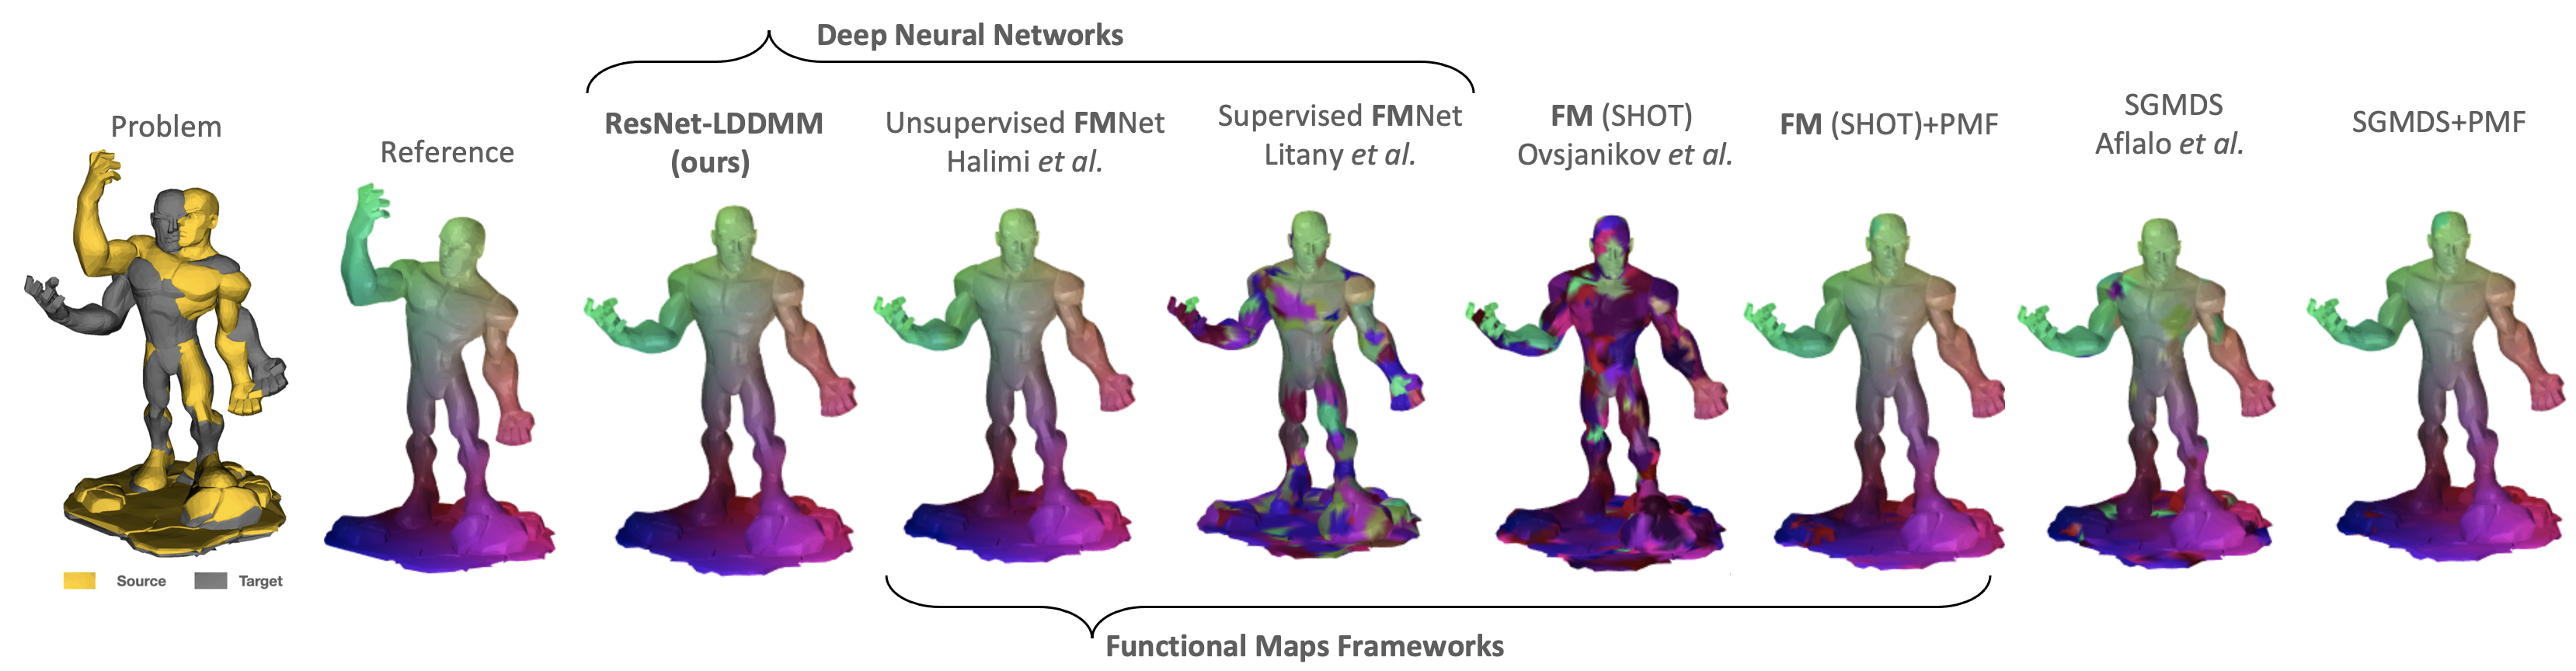
\includegraphics[width=\linewidth]{Figs/ArtistComparison-2.png}
\vspace{-0.8cm}
  \caption{Qualitative comparison of ResNet-LDDMM (third column) to state-of-the-art approaches including \textit{Functional Maps (FM)} framework and Supervised and Unsupervised \textit{FM}Net on human-like artistic models (the six last registration results are previously reported by Halimi \etal in \cite{halimi2019unsupervised}).}
   \label{Fig:Artist}
\end{figure*}

\subsection{The \textit{Functional Maps} Framework}
\label{sec:FunctionalMaps}

Rather than matching individual points, which remains a hard problem, a family of approaches propose to match scalar functions over the shapes. Among them, the \textit{Functional Maps} framework introduced by Ovsjanikov \etal in \cite{ovsjanikov2012functional}. The key idea is to find shape-to-shape correspondence using real-valued (descriptor) functions. Candidate function maps are ideally invariant under the transformations to filter out. Basically, a shape map lifts to a linear operator mapping the function spaces. Then, a compact representations of functional maps are obtained by projection of the linear operator in a predefined basis (the \textit{Laplace-Beltrami} eigenbasis (LBO) is a typical choice). The fundamental problem is to obtain such suitable descriptors.

FMNet introduced in \cite{litany2017deep} learns descriptors to achieve the correspondence. So that, the output of FMNet is a dense vector-valued descriptor, calculated on each of the input shapes. Recently, in \cite{halimi2019unsupervised} the first unsupervised learning scheme was proposed. Dense correspondence is obtained by minimizing pair-wise geodesic distance distortion computed on the pair of shapes. This approach could be viewed as the fusion of GMDS \cite{aflalo2016spectral} and an unsupervised version of FMNet \cite{litany2017deep}. The Deep Learning Functional Maps approaches require an initialization with pre-computed descriptors typically SHOT \cite{tombari2010unique}. In \cite{halimi2019unsupervised}, the descriptors learned from correspondences, are replaced by geometric invariant descriptors (matrices of all pairwise geodesic distances). More recently, inspired by FMNet (unsupervised regime) and 3D-CODED (supervised regime), a deep geometric functional map (\ie an hybrid approach) was proposed in \cite{donati2020deep}. Here, the network performs a feature-extraction and learns directly from raw shape geometry, combined with a novel regularized map extraction layer and loss, based on the functional map representation. This hybrid approach is less dependant to the data size in the training set compared to the 3D-CODED approach \cite{groueix20183d}. Other approaches first map the shapes to a canonical space (\eg \cite{ovsjanikov2010one}), then solve for the correspondence between obtained parametric representations, blend across such maps \cite{kim2011blended}, or compute multiple near-isometric dense correspondences \cite{ren2020maptree}, rather than optimizing for a single solution. 

%\textcolor{red}{Despite their effectiveness by learning descriptors \cite{donati2020deep} or grounding on predefined isometric descriptors \cite{halimi2019unsupervised}, the Functional Maps approach remains sensitive to the quality of the input shapes (\eg presence of noise and missing data \cite{rodola2017partial}). They are also restricted to handle near-isometric transformations. }

%
 

%\subsection{Deep Neural Network Methods}
%\label{sec:DLapproaches}

%Most recent end-to-end unsupervised deep learning diffeomorphic registration approaches are inspired from the SVF framework. Indeed, they make use of spacial transformer networks (or STNs), first introduced in \cite{jaderberg2015spatial}, to warp the source (moving image) to the target (fixed image) by optimizing a loss function including both an image similarity term and a regularization on the transformations term. One pioneering approach is called \textit{VoxelMorph} and works on (structured) 3D medical images \cite{dalca2018unsupervised, dalca2019unsupervised}. The Network, a UNet, consists of two steps. First, it approximates posterior probability parameters representing the velocity field mean and variance using a convolutional encoding-decoding scheme. Second, obtained velocity fields are transformed into diffeomorphic transformation using differentiable squaring and scaling integration layers. Similarly, Krebs \etal proposed in \cite{krebs2019learning} to use a conditional variational autoEncoder (\textit{CVAE}) to infer a low-dimensional probabilistic deformation model under constraints making the transformations symmetric and diffeomorphic. The main idea is to build the target by warping the source image, where the latent space encodes deformations. Again, successive differentiable squaring and scaling layers, as previously used in \cite{dalca2018unsupervised}, generate diffeomorphic transformations. The decoder extracts velocities and diffeomorphisms at different scales and a Gaussian smoothing layer is applied on the filter maps (latent variables) to smooth the initial velocity. Taking advantage of symmetric approaches, Mok and Chung proposed in \cite{mok2020fast} a symmetric diffeomorphic neural network (\textit{SDNN}) which is an unsupervised symmetric image registration method which maximizes the similarity between images within the space of diffeomorphic maps and estimates both forward and inverse transformations simultaneously. On top of this, they proposed a selective Jacobian determinant regularization that imposes a local orientation, consistency constraint on the estimated deformation fields. Also, inspired by the SVF framework, Bone \etal have proposed in \cite{bone2019learning} a diffeomorphic autoencoder (\textit{DAE}). In \cite{shen2019networks}, Shen \etal have proposed a deep-learning framework which combines affine registration and a vector momentum-parameterized  stationary velocity field (\textit{vSVF}). Under the vSVF approach, the goal is also to solve a stationary ODE that represents a one-parameter subgroup of diffeomorphisms. The integration is achieved via multiple scaling and squaring layers. The way to accommodate a convolutional neural network to compute vSVF, under a supervised learning scheme, was first proposed in \cite{rohe2017svf}. Taking a slightly different direction and inspired by the work of Vialard \etal \cite{vialard2012diffeomorphic}, Niethammer \etal have proposed in \cite{niethammer2019metric} to learn a spatially-varying regularizer. They built their unsupervised registration model on top of \textit{vSVF} \cite{arsigny2006log}. Their approach jointly optimizes the regularizer (parameterized by a deep CNN) and the registration parameters of the \textit{vSVF} model. To allow much freedom, Shen \etal have proposed in \cite{shen2019region} a Region-specific Diffeomorphic Metric Mapping (\textit{RDMM}) to allow for spatially-varying regularization. Unlike spatially-invariant regularizers, spatially-varying regularization allows anticipating different levels of deformations at different image locations. It was observed experimentally that \textit{RDMM} may locally exhibit stronger deformations than \textit{LDDMM} or \textit{vSVF}. \\

\subsection{Link between ResNets and Geometric Flows}
\label{sec:LinkResNet-LDDMM}

The interpretation of ResNets as transformations on the data space is not new. For example, \cite{NIPS2017_0ebcc77d} studies the induced change on the Riemannian metric of the deformations, while \cite{ruthotto2019deep} interprets convolution of images as partial differential operators, and each residual layer as a forward Euler scheme. From there, the recent paper \cite{rousseau2020residual} of Rousseau \etal uses for the first time the idea that ResNets actually generate diffeomorphisms on the space in which the data lives (or at least, bi-lipshitz maps). The paper both deepens the theoretical understanding of ResNets and provides improved algorithms for the classification of data. In the same context, L. Younes have introduced a diffeomorphic learning paradigm in which training data is transformed by a diffeomorphic transformation (defined in high dimensional space) before the final prediction \cite{younes2019diffeomorphic}. Importantly, an Optimal Control formulation of the learning algorithms was derived as well as the importance of such smooth and invertible transformations in generative models was discussed. 

The main difference between our approach and that of  \cite{rousseau2020residual}, which also defines diffeomorphisms, is that we do not build diffeomorphisms on the data space (that is, the space $\real^{n\times 3}$ in which the whole shape lives), but on the ambient space $\real^3$. Then, this transformation is applied separately to each point $x_i, i=1,\dots,n$ of the shape. This ensures the preservation of the topology of the shape. This is partly why we did not include surface convolution layers with filter size $>1$, for example. Such layers would still yield diffeomorphisms in  $\real^{n\times 3}$ as per \cite{rousseau2020residual}, but those transformations would not translate into well-defined transformation of $\real^3$.

%\textcolor{red}{To our knowledge, ResNet-LDDMM is the first to consider non-rigid registration using Residual networks. }

\subsection{Contributions and Paper Organization}

In this work, we propose a novel joint geometric-neural networks framework for diffeomorphic registration of 3D point clouds (and meshed surfaces). Our formulation differs in several aspects from previous deep learning approaches. It is also much more in line with LDDMM methods than \cite{rousseau2020residual}. The paper's contributions are summarized as follows,

$\hookrightarrow$ We introduce a Riemannian-like framework (thus, a length space), for deforming, registering and comparing 3D shapes, by revisiting the original LDDMM framework using Deep Residual Networks. Up to our knowledge, despite the similarity to previous interpretations of Residual Networks as flow of diffeomorphisms, our work is the first to demonstrate these ideas on 3D shape registration problems.
    
$\hookrightarrow$ Our ResNet-LDDMM predicts time-dependent, regular and smooth velocity fields (the endpoint of the flow is the desired diffeomorphic transformation). It brings a novel regularization driven by the time-integrated kinetic energy (or the geometric norm of the control, \ie the velocity fields). We demonstrate that just like in LDDMM, ResNet-LDDMM does generate (essentially) a diffeomorphism of the ambient space $\real^3$ itself, instead of just on the data space as in \cite{rousseau2020residual}.
    
$\hookrightarrow$ Appropriately applying the ReLU activation function to predict velocity fields, we reveal how each time-step of our ResNet-LDDMM divides the space $\real^3$ into multiple polytopes (\ie, unbounded polyhedra) in which optimal affine velocity fields are computed. This ensure more flexibility in the registration while maintaining diffeomorphic properties. Up to our knowledge, this geometric interpretation has not been described so far, although some similar interpretations have been suggested in \cite{rousseau2020residual} and \cite{younes2019diffeomorphic} in the context of diffeomorphic learning. 

$\hookrightarrow$ We report competitive results in comparison to the original LDDMM framework, to recent non-rigid point-clouds registration approaches, to different variants of the \textit{Functional Maps} framework and to supervised Deep Learning techniques. As a first experimental illustration of our non-rigid registration approach, we report in Fig.\ref{Fig:Artist} results on humanoid-like meshes and compare with state-of-the-art methods. This figure highlights the limitation of supervised learning techniques \cite{litany2017deep} to generalize on new deformations, as discussed in \cite{halimi2019unsupervised}. In addition, as experimented in \cite{halimi2019unsupervised}, Functional Maps require, in general, a time-consuming post-processing refinement step \cite{vestner2017efficient}, called Product Manifold Filter (PMF), and an initialization step using SHOT descriptors. More efficient and accurate refinement methods have been developed recently. For example, in \cite{ezuz2017deblurring} a new method for map deblurring was proposed, by introducing a smoothness prior on the reconstructed map which results in better maps, especially when the shapes are not isometric. Taking a different direction, Melzi \textit{et al.} showed in \cite{melzi2019zoomout} that a higher resolution map can be recovered from a lower resolution one through a remarkably simple and efficient iterative spectral up-sampling technique. Consequently, a simple and efficient method for refining maps or correspondences by iterative upsampling in the spectral domain have been proposed. More recently, Pai \textit{et al.} introduced in \cite{pai2021fast} a method which combines the simple and concise representation of correspondence using FMs with the matrix scaling schemes from computational optimal transport. The approach improves accuracy and bijectivity of correspondences.

While our ResNet-LDDMM operates on the original point clouds, \textit{Functional Maps} approaches require to define (\eg \cite{halimi2019unsupervised}) or to lean (\eg \cite{litany2017deep}) a descriptor function, which make them conceptually different. The rest of the paper is organized as follows. In Sec. \ref{sec:ResNet-LDDMM}, we describe our ResNet-LDDMM framework from both geometric and (unsupervised learning) neural networks perspectives. How ResNet-LDDMM naturally builds diffeomorphic transformations between shapes is formally elaborated in Sec. \ref{sec:Diffeos}. Furthermore, we provide a geometric description of the velocity fields accompanied by a qualitative interpretation on the registration methodology behind ResNet-LDDMM. Sec. \ref{sec:Experiments} is dedicated to multiple experiments. Some concluding remarks and perspectives are drawn in Sec. \ref{sec:Conclusion}.

%\textcolor{blue}{\textbf{--} On different internal anatomical organs, we study the performance of our ResNet-LDDMM in comparison with LDDMM . We show its superiority in some cases. We compare to other non-rigid registration approaches as N-ICP \cite{amberg2007optimal}, RPTS \cite{li2018robust}, SVR-$\ell_0$ \cite{guo2015robust} and QNS \cite{Yao_2020_CVPR} on body shapes. We highlight in particular its behavior in the presence of noise and missing data.}

%\textcolor{blue}{\textbf{--} While Deep Functional Maps, \eg \cite{litany2017deep,donati2020deep} in supervised regime, train/extract a descriptor as a real-valued function, our network computes flows of velocity fields under an unsupervised regime.} 



\begin{figure*}
  \centering
   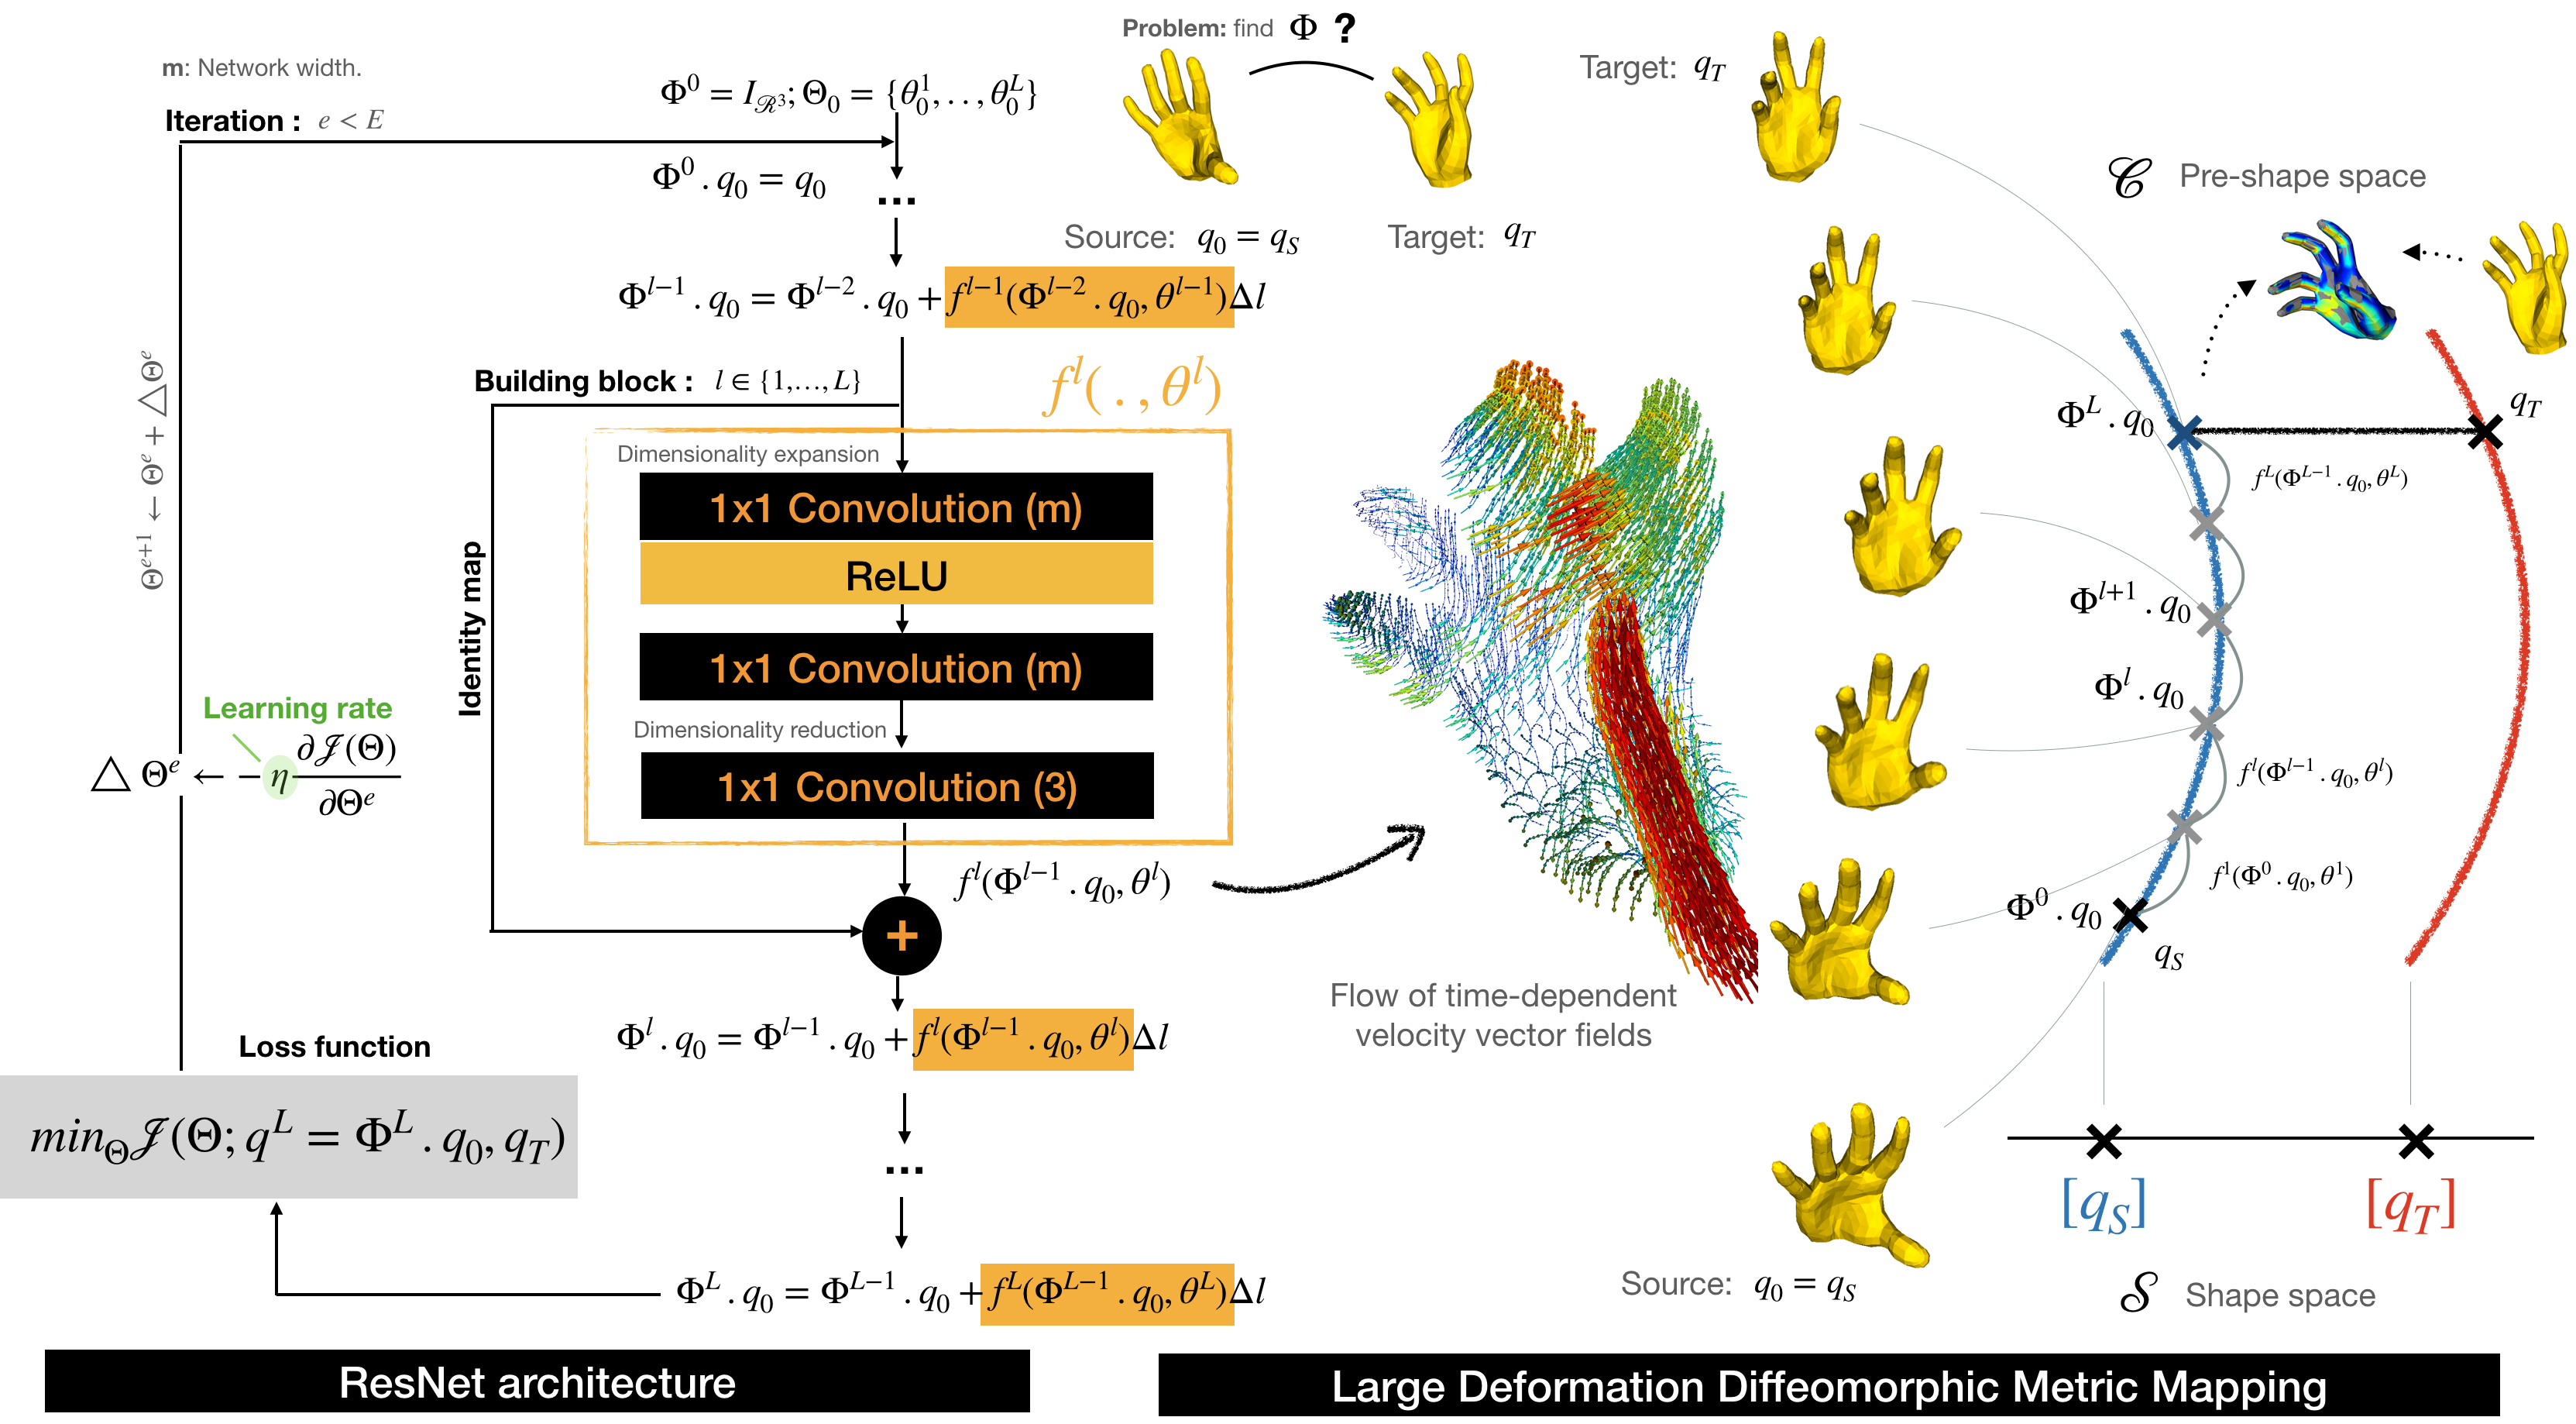
\includegraphics[width=\linewidth]{Figs/Overview-ResNet-LDDMM-3.png}
%\vspace{-0.3cm}
  \caption{Overview of our joint ResNet-LDDMM diffeomorphic registration framework -- the ResNet architecture is shown on the left, comprising of an ensemble of successive two-layers ReLU networks followed by a dimensionality reduction layer (the ensemble is called a building block). Each predicts a time-dependent velocity field $f^l(.,\theta^l)$. On the right, we show the flow of obtaining velocity fields and diffeomorphisms $\Phi^l$ applied to the source shape, including the end-point $\Phi^L$, achieved by integration. In Computational Anatomy (\eg \cite{miller2004computational}), it is assumed that observations of the same anatomical organ are elements of a common shape Orbit, so that $[q_S]$ and $[q_T]$ coincide. The Network's width $m$ is the number of filters.}
   \label{Fig:Overview}
\end{figure*}